\section{Evaluation}

\subsection{Experimental Setup}

We ran real DNS traces on a simulated DDNS network
of servers to measure load balancing. We set up a
Chord ring of 1000 nodes and seeded the ring with 
real DNS data. Then performed lookup requests.

\subsection{Load Balance}

%\includegraphics[angle=270,width=3.5in]{figures/ok.fetch.eps}
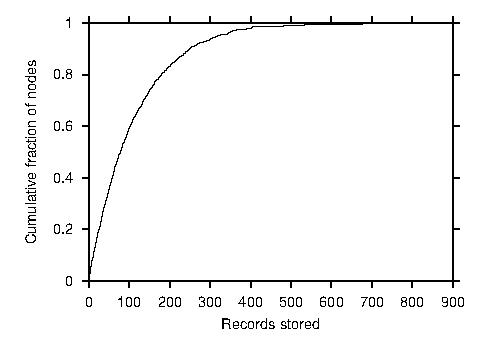
\epsfig{file=figures/ok.store.eps,angle=270,width=3.5in}
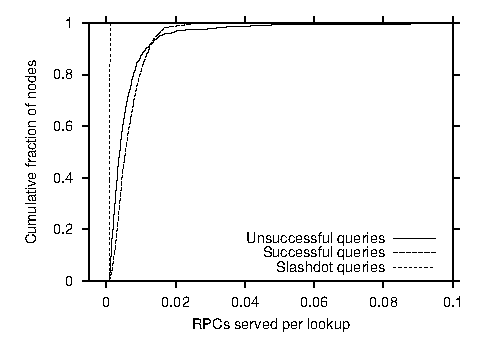
\epsfig{file=figures/both.fetch.eps,angle=270,width=3.5in}
\epsfig{file=figures/slashdot.fetch.eps,angle=270,width=3.5in}

Do a measure of how long it takes to converge to good load 
balancing when there is a burst of lookups for 1 (or more)
popular names. Compare that to the slashdot effects now.

%\subsubsection{Latency}

%We cannot perform a fair measurement of latency so we will do an
%analysis based on counting number of hops between servers
%and combining that with real latency to current root DNS servers.

%XXAdding keys to resource records make them bigger
%XXPublic key cryptography is an expensive operation. 
%DDNS computes pub keys every time.

%DDNS is not going to disappear without an answer for a lookup,
%unlike in the current DNS. So we can't really compare this, but should
%mention about it.
